\subsection{Output View Models}
\begin{center}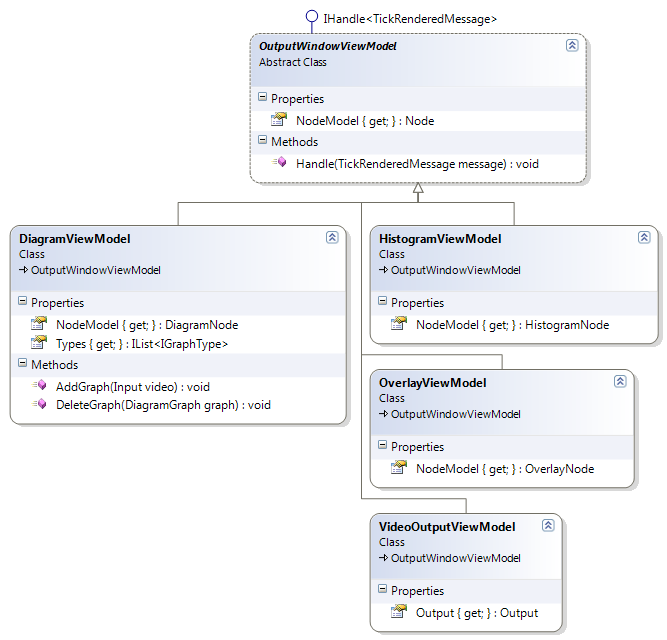
\includegraphics[scale=0.7]{YuvKA.ViewModel/outputs.png} \\
\end{center}
%< Beschreibung des Subsystems >

\subsubsection{YuvKA.ViewModel.OutputWindowViewModel}

\begin{verbatim}
public abstract	class OutputWindowViewModel : IHandle<FrameRenderedMessage>
\end{verbatim}

\paragraph{Beschreibung}~\\
%< Beschreibung der Klasse >

\paragraph{Typmember}
\begin{itemize}

\property{NodeModel}
	\begin{verbatim}
public Node NodeModel { get; }
	\end{verbatim}
%	<Membererklärung>


\method{Handle}
	\begin{verbatim}
public virtual void Handle(FrameRenderedMessage message)
	\end{verbatim}
%< Methodenerklärung >


\end{itemize}

\subsubsection{YuvKA.ViewModel.DiagramViewModel}

\begin{verbatim}
public class DiagramViewModel : OutputWindowViewModel
\end{verbatim}

\paragraph{Beschreibung}~\\
%< Beschreibung der Klasse >

\paragraph{Typmember}
\begin{itemize}

\property{NodeModel}
	\begin{verbatim}
public Node NodeModel { get; }
	\end{verbatim}
%	<Membererklärung>

\property{Types}
	\begin{verbatim}
public IList<IGraphType> Types { get; }
	\end{verbatim}
%	<Membererklärung>


\method{AddGraph}
	\begin{verbatim}
public void AddGraph(Input video)
	\end{verbatim}
%< Methodenerklärung >

\method{DeleteGraph}
	\begin{verbatim}
public void DeleteGraph(DiagramGraph graph)
	\end{verbatim}
%< Methodenerklärung >

%%%%% Interne Klasse Input Hier bitte. %%%%%

\end{itemize}

\subsubsection{YuvKA.ViewModel.HistogramViewModel}

\begin{verbatim}
public class HistogramViewModel : OutputWindowViewModel
\end{verbatim}

\paragraph{Beschreibung}~\\
%< Beschreibung der Klasse >

\paragraph{Typmember}
\begin{itemize}

\property{NodeModel}
	\begin{verbatim}
public Node NodeModel { get; }
	\end{verbatim}
%	<Membererklärung>

\end{itemize}

\subsubsection{YuvKA.ViewModel.OverlayViewModel}

\begin{verbatim}
public class OverlayViewModel : OutputWindowViewModel
\end{verbatim}

\paragraph{Beschreibung}~\\
%< Beschreibung der Klasse >

\paragraph{Typmember}
\begin{itemize}

\property{NodeModel}
	\begin{verbatim}
public Node NodeModel { get; }
	\end{verbatim}
%	<Membererklärung>

\end{itemize}

\subsubsection{YuvKA.ViewModel.VideoOutputViewModel}

\begin{verbatim}
public class VideoOutputViewModel : OutputWindowViewModel
\end{verbatim}

\paragraph{Beschreibung}~\\
%< Beschreibung der Klasse >
